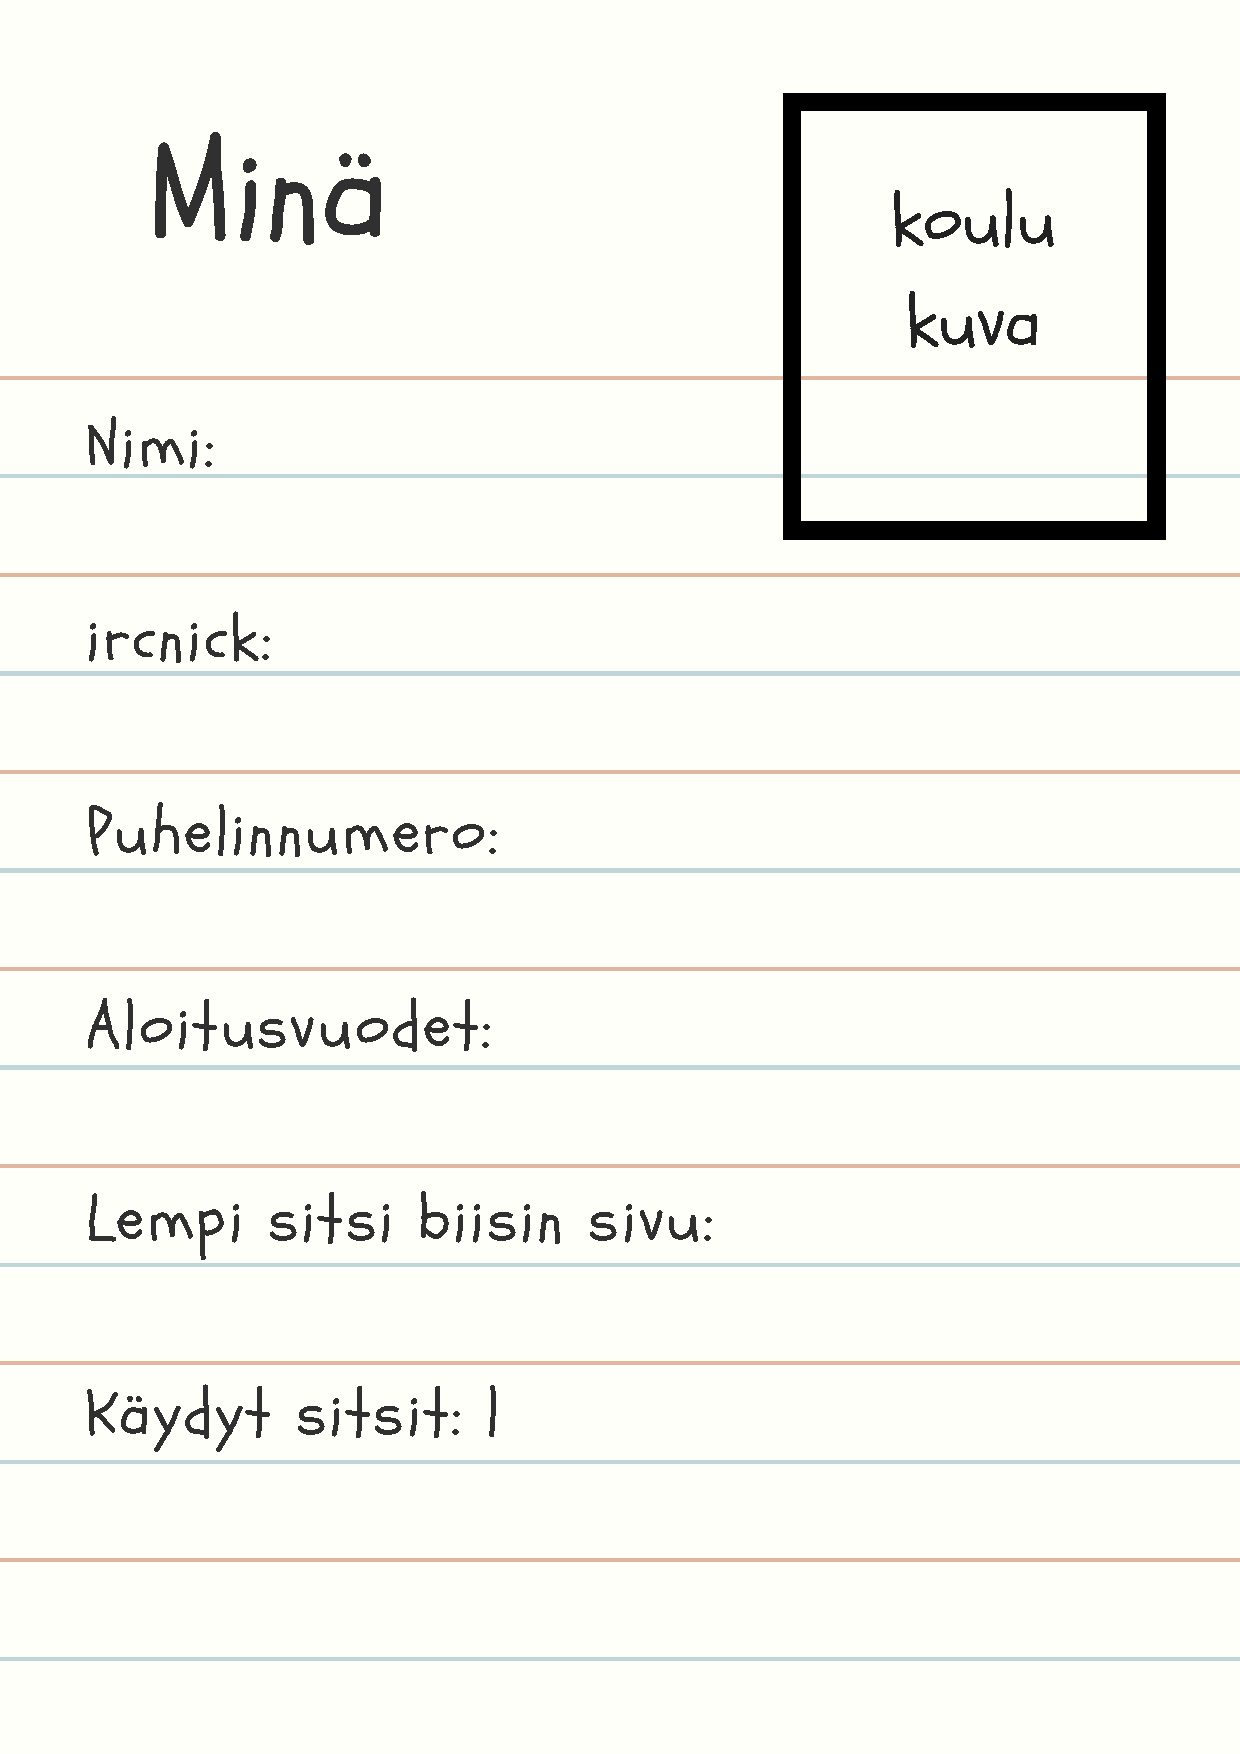
\includepdf{graphics/Kamukirja.pdf}


\newpage
\begin{figure}[t]
\vspace{-0.8cm}
\centering
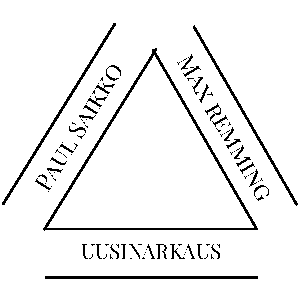
\includegraphics[scale=0.82]{graphics/tekijat.pdf}
\vspace{-0.8cm}
\end{figure}

\noindent
\textbf{Julkaisija:} \\
\noindent
TKO-äly ry \\

\noindent
\textbf{Laulukirjavastaavat:} \\
\noindent
Julius Uusinarkaus, Maximilian Remming \\

\noindent
\textbf{Taittosofta:} \\
\noindent
Paul, Max \\

\noindent
\textbf{Lauluja keräsi:} Jonne Huotari, Juho Kostet, Felix Lindholm, Henri Malkki, Jussi Maristo, Eetu Mattila, Mikko Rinta-Homi, Ville-Veikko Saari, Julius, Max, Paul\\

\noindent
\textbf{Kategoriasivut:} Hugo Holmqvist, Mauri Karlin, J, Paul \\

\noindent
\textbf{Oikoluku, läpilaulu:} Valentin Abramenkov, Ada Hyvärinen, Sami Lindqvist, Markus Riskumäki, Nico Roos\\

\noindent
\textbf{Kirjojen nouto:} Kimmo Kulmala, Miia Rämö

\noindent
\textbf{Suurkiitokset:} Google Sheets, Python, \LaTeX \\

\noindent
\textbf{Painos:} 5/2017 -- 520 kpl -- Tallinna Raamatutrükikoda \\
\newpage

\afterpage{\blankpage}
\begin{figure}[h!]
\centering

\includegraphics[scale=0.4]{graphics/logo.png}
\end{figure}

\newpage

\textbf{Esipuhe}
\\

Matemaatikot latoivat laulukirjan käsin latexilla, perinteitä kunnioittaen.
Valtiotieteilijät toisaalta pitkillä kokouksilla. Itse kunnioitimme
tietojenkäsittelijöiden perinteitä. Laulu\-kirjamme on ladottu excelistä
python-scriptillä \LaTeX{}iin. Sopivalla määrällä mee\-mi\-taikaa. Niin, ja tätä on työstetty 6 vuotta.

Laulukirja on paljon enemmän kuin laulukirja. Kirja on tieten\-kin hyvä työkalu
sitseillä, mutta sen aito tarkoitus on jäädä ra\-por\-tik\-si menneestä. Laulukirjaan
kerääntyy satoja viestejä, rivouksia ja muita tervehdyksiä, nykyisiltä ja
menneiltä ystäviltä. Laulukirja kuluu, mutta paranee iän myötä. Teimme tämän
laulukirjan sel\-lai\-sek\-si, että siitä on sinulle vielä iloa pitkään. Siitä tulee
jokaisen sitsin jälkeen enemmän omannäköisesi. Voit lisätä puuttuvat lempi\-laulusi DLC-sivulle tai tyhjille sivuille.
Kirjassa on myös varmasti lauluja jotka eivät tule olemaan seuraavassa
kirjassa, eivätkö olleet edellisessä. Uskomme kuitenkin että tämä kirja on oiva
ajankuva nykyisistä toimijoista ja kulttuurista.

Kirjassa on muutamia käyttämistä helpottavaa erikoisuutta. Sivun yläkulmassa on laulunumero, jotta
voit löytää sitsitilanteessa laulun mahdollisimman nopeasti. Indeksiin on merkitty myös lau\-luil\-le vaihtoehtoisia nimiä.

We wanted to make the book accessible, and actually useful, even if you don’t
speak Finnish. We put together as many “fun to drink together, or while drunk”-songs
in english as we could. We tried to make this the ultimate combination of a
sophisticated traditional song book, and meme magic. I think we did well.
\\
\\
Hyvää vappua!

\vfill
\textit{Julius ja Max}

\newpage
\blankpage
